% ML: proc neni tento text v 6-kapitola.tex ?
\chapter{Konvenční prostředky a polygonizace}
\label{chap:konvencni prostredky a polygonizace}
Existuje celá řada konvenčních nástrojů, kterými lze řešit
polygonizaci. Oblast GIS je známá značným množstvím kvalitních
nástrojů s otevřeným zdrojovým kódem. Můžeme tak nalédnout do
implementace jednotlivých softwarových řešení. Výhodou je i velká
% ML: komercni neni presne, asi "proprietarni" (i kdyz to nezni
% cesky), komerce je spojena i s open source...
komunita, která vždy ochotně poradí. Mimo jiné jsou zde i komerční
zástupci, kteří nám možnost nahlédnout do zdrojového kódu zpravidla
nenabídnou. Zato by nám měli poskytovat uživatelskou podporu, za
kterou zákazník samozřejmě platí koupí softwaru.
	
Mohlo by se zdát, že nástrojů existuje celá řada, tak proč vytvářet
nástroj nový? Jedná se zde především o spolehlivost a
jednoduchost. Jak u komerčních, tak u open source nástrojů je s
nadsázkou téměř tradicí, že po přechodu na vyšší verzi nějaké
komponenty přestanou fungovat a končí na neočekávaných
chybách. Výjimkou nejsou ani nástroje pro polygonizaci.
	
Zmíníme zde tedy nejvýznamější zástupce z oblasti GIS a ukážeme, které
nástroje z těchto softwarů lze pro polygonizaci využít.
	
\section{ArcGIS Desktop}
ArcGIS je vyvíjený společností Esri, v současné době se jedná o jeden
z nejvyužívanějších nástrojů v oblasti GIS. Jedná se o placený
% ML: co presne zname "nekomercni", napr. neziskovka?
% ML: chybi reference...
software, za který nekomerční uživatel v současné chvíli zaplatí 100
dolarů ročně. Používat tento nástroj tedy pouze pro polygonizaci by
bylo nesmyslné, ovšem pokud uživatel již tímto softwarem disponuje, je
toto jedna z možností.
	
\subsubsection{Feature to Polygon}
\textit{Feature to Polygon} je nástroj sloužící pro tvorbu
polygonů. Jako vstupní data mohou být použity linie i
polygony. Výstupní polygony z tohoto nástroje na testovacích datech
byli korektní, ovšem při větším množství vstupních linií testovaný
nástroj končil chybou. Nutno podotknout, že u různých verzí softwaru
se může nástroj chovat jinak.

\begin{figure}[h]
  \centering
  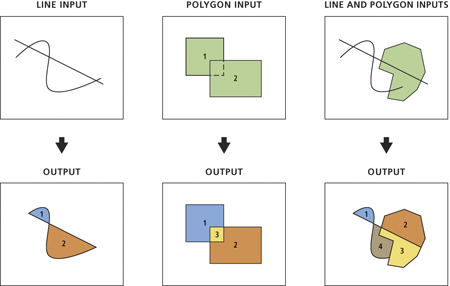
\includegraphics[width=10cm]{./pictures/5_1/feature_to_polygon.png}
  \caption{Ilustrace vstupu a výstupu nástroje Feature to Polygon. Převzato z~\cite{arcgis}.}
  \label{fig:feature_to_polygon}
\end{figure}

% ML: tento obrazek zapadne zbytecne daleko do textu
\begin{figure}[h]
  \centering
  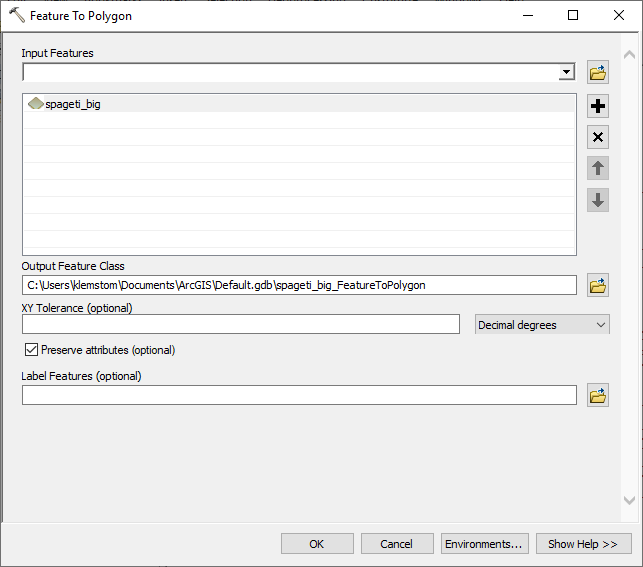
\includegraphics[width=10cm]{./pictures/5_1/feature_to_polygon-1.png}
  \caption{Rozhraní nástroje Feature to Polygon v softwaru ArcGIS Desktop.}
  \label{fig:feature_to_polygon-1}
\end{figure}


\section{QGIS Desktop}
Přímým konkurentem softwaru ArcGIS Desktop je bezpochyby vydařený QGIS
Desktop. Jedná se o nástroj vyvíjený komunitou pod záštitou OSGeo. Je
šířen pod copyleftovou licencí \textit{GNU General Public License},
tudíž máme volný přístup ke zdrojovému kódu aplikace dostupnému v
online repozitářích. To nám umožňuje nahlížet do výpočetních
algoritmů, které jsou v případě QGIS psány v programovacím jazyce
\textit{C++} a \textit{Python}, narozdíl od komerčních nástrojů, které
si implementaci často chrání. Výstup z nástroje byl opět validní. Na
rozdíl od nástroje z ArcGIS Desktop se ovšem podařilo zpracovat i
%% ML: hodil by odkaz do dodatku, kde budes mit realne porovnani
%% (jinak je to pouze tvrzeni bez podlozenych dat)
větší množství dat.

\subsubsection{Polygonize}
Nástroj Polygonize je od verze 3.12 napsán v \textit{C++}, v
předchozích verzích QGIS Desktop byl zakomponován formou pluginu
psaného v jazyce Python. Využívá metod knihovny GEOS. Důležitý rozdíl
oproti nástroji z ArcGIS Desktop je že na vstupu neakceptuje jiné
prvky než linie~\cite{QGIS_software}.

% ML: tento obrazek zapadne zbytecne daleko do textu
\begin{figure}[h]
  \centering
  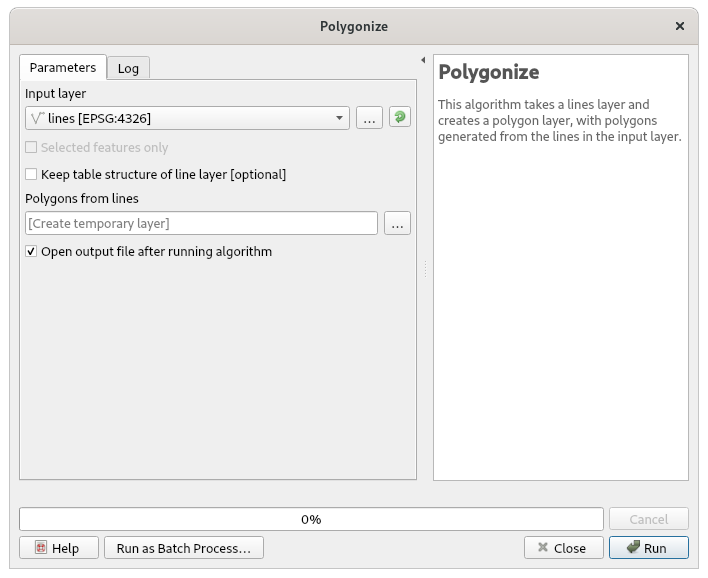
\includegraphics[width=10cm]{./pictures/5_1/polygonize.png}
  \caption{Rozhraní nástroje Polygonize v softwaru QGIS Desktop.}
  \label{fig:polygonize}
\end{figure}

\section{PostGIS}
Obdobně byl testován i nástroj PostGIS. Zde už se nejedná o
desktopovou aplikaci, jako tomu bylo u výše testovaných
softwarů. PostGIS je nadstavba pro objektově-relační databázi
PostgreSQL. Jedná se tedy o rozšíření databáze o podporu
geo\-grafických objektů a funkcí. Je často využíván k uchování
geografických dat a analýz nad nimi. Nutno podotknout, že PostGIS
využívá pro většinu svých o\-pe\-ra\-cí taktéž knihovnu \textit{GEOS}
psanou v programovacím jazyce \textit{C++}, kterou následně poskytuje
uživateli přes standardní dotazovací jazyk SQL.
	
Postup polygonizace zde bude o něco složitější. Budeme nuceni
polygonizaci rozdělit do dvou kroků, jak bylo řečeno v
kapitole~\ref{chap:reserzepouzivanychalgoritmu}. Nejprve se tedy
zaměříme na doplnění průsečíků linií a poté provedeme vlastní
polygonizaci. Pro doplnění průsečíku linií nám PostGIS nabízí hned dvě
možnosti.
	
\subsubsection{Funkce \textit{ST\_UnaryUnion}}
První z možností je využít funkci \textit{ST\_UnaryUnion}. Tato funkce
rozpouští linie tak, že sdílí maximálně koncový bod s jinými
liniemi. Tímto způsobem můžeme připravit podkladové linie pro
následnou polygonizaci. Nevýhoda této funkce je ovšem v její časové
složitosti. Oproti druhé možnosti, tedy funkci \textit{ST\_Node},
dosahuje značně vyšších časů pro výpočet~\citep{PostGIS_software}.
	% select st_unaryunion(st_collect(st_linemerge(geom))) from spageti_small;
	
\subsubsection{Funkce \textit{ST\_Node}}
Druhá možnost a alternativa funkce \textit{ST\_UnaryUnion} je funkce
\textit{ST\_Node}. Tato funkce taktéž rozpojuje linie v
průsečících. Nicméně oproti předchozí zmíněné pracuje v mnohem
kratších časech. Výhodou obou těchto funkcí může být možnost pracovat
s 3D daty~\cite{PostGIS_software}.

% https://trac.osgeo.org/geos/ticket/962

\subsubsection{Funkce \textit{ST\_Polygonize}}
Pokud máme průsečíky doplněny, můžeme přistoupit k vlastní tvorbě
polygonů. K tomu nám poslouží funkce \textit{ST\_Polygonize}
využívající metod knihovny GEOS. Výstupem této funkce je pak
geometrická kolekce obsahující polygony~\cite{PostGIS_software}.

\begin{figure}
\begin{minted}
{postgresql}
SELECT st_polygonize(lines_nodded.geom) AS geom
FROM (
        SELECT st_node(st_collect(st_linemerge(geom))) AS geom
        FROM lines_small
    ) AS lines_nodded
\end{minted}
\caption{Příklad tvorby polygonů v PostGIS.}
\label{fig:SQL_polygonize}
\end{figure}


	
	
	
	